\newcommand{\asyncawait}{\texttt{async/await}}

\section{Tokio}\label{sec:tokio}
Asynchronous programming in Rust requires an asynchronous run-time to poll the futures produced from \texttt{async}
functions.
One of the first run-times was Tokio~\citep{tokiocommunity_tokioasynchronousruntime_}, and has become the de-facto standard
asynchronous runtime for Rust.
Tokio existed prior to \asyncawait{} syntax as a runtime for futures directly.
At the beginning of the project, Rust was still stabilising its \asyncawait{} syntax~\citep{withoutboats_asyncawaitnotation_},
so there was no
complete and stable implementations of the asynchronous runtime.
The closest was Tokio's unstable implementation, which was stabilised soon after Rust stabilising
\asyncawait{}.
Now there exists multiple asynchronous run-times with the three main ones being Tokio, async-std and actix-rt.
Actix-rt provides an asynchronous runtime intended for use with the actor design pattern.
This API will not follow this pattern, so will not use actix-rt.
Async-std is a library which is modelled on Rust's own standard library with the intention of translating the standard
library to be \asyncawait{} compatible.
Where Tokio is intended to be a fully-featured asynchronous programming platform, async-std is a port of the existing
standard library.
Ultimately, Tokio is a more mature library with a much larger user base, so Tokio will be used over async-std.

%What did you do to implement this idea, and what technical achievements did you make?
%\section{Guidance}
%You can't talk about everything. Cover the high level first, then cover important, relevant or impressive details.
%
%
%
%\section{General points}
%
%These points apply to the whole dissertation, not just this chapter.
%
%
%
%\subsection{Figures}
%\emph{Always} refer to figures included, like Figure \ref{fig:relu}, in the body of the text. Include full, explanatory captions and make sure the figures look good on the page.
%You may include multiple figures in one float, as in Figure \ref{fig:synthetic}, using \texttt{subcaption}, which is enabled in the template.
%
%
%
%% Figures are important. Use them well.
%\begin{figure}
%    \centering
%    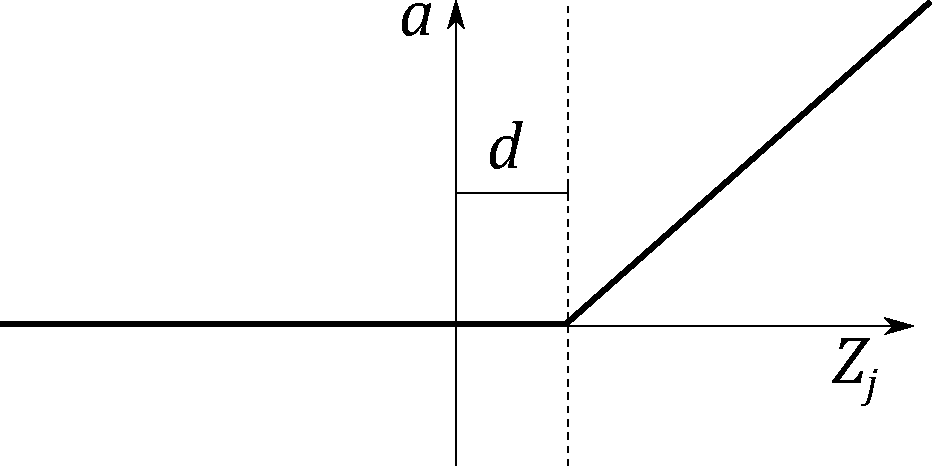
\includegraphics[width=0.5\linewidth]{images/relu.pdf}
%
%    \caption{In figure captions, explain what the reader is looking at: ``A schematic of the rectifying linear unit, where $a$ is the output amplitude,
%    $d$ is a configurable dead-zone, and $Z_j$ is the input signal'', as well as why the reader is looking at this:
%    ``It is notable that there is no activation \emph{at all} below 0, which explains our initial results.''
%    \textbf{Use vector image formats (.pdf) where possible}. Size figures appropriately, and do not make them over-large or too small to read.
%    }
%
%    % use the notation fig:name to cross reference a figure
%    \label{fig:relu}
%\end{figure}
%
%
%\begin{figure}
%    \centering
%    \begin{subfigure}[b]{0.45\textwidth}
%        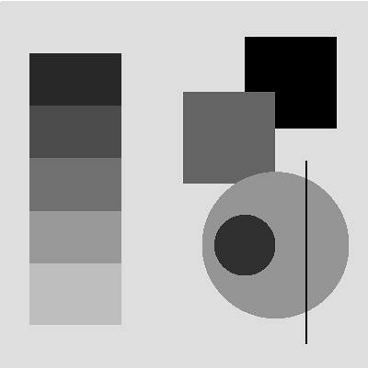
\includegraphics[width=\textwidth]{images/synthetic.png}
%        \caption{Synthetic image, black on white.}
%        \label{fig:syn1}
%    \end{subfigure}
%    ~ %add desired spacing between images, e. g. ~, \quad, \qquad, \hfill etc.
%      %(or a blank line to force the subfigure onto a new line)
%    \begin{subfigure}[b]{0.45\textwidth}
%        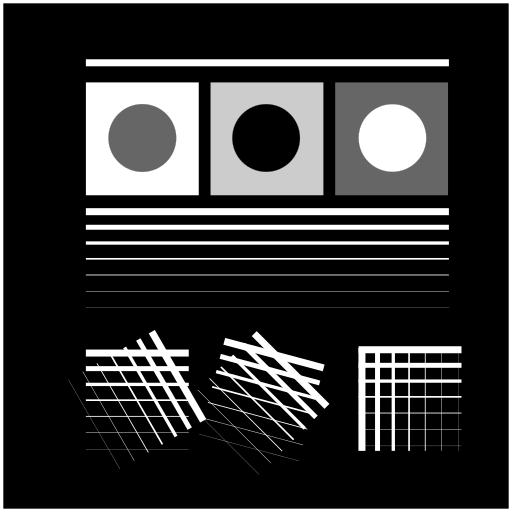
\includegraphics[width=\textwidth]{images/synthetic_2.png}
%        \caption{Synthetic image, white on black.}
%        \label{fig:syn2}
%    \end{subfigure}
%    ~ %add desired spacing between images, e. g. ~, \quad, \qquad, \hfill etc.
%    %(or a blank line to force the subfigure onto a new line)
%    \caption{Synthetic test images for edge detection algorithms. \subref{fig:syn1} shows various gray levels that require an adaptive algorithm. \subref{fig:syn2}
%    shows more challenging edge detection tests that have crossing lines. Fusing these into full segments typically requires algorithms like the Hough transform.
%    This is an example of using subfigures, with \texttt{subref}s in the caption.
%    }\label{fig:synthetic}
%\end{figure}
%
%\clearpage
%
%\subsection{Equations}
%
%Equations should be typeset correctly and precisely. Make sure you get parenthesis sizing correct, and punctuate equations correctly
%(the comma is important and goes \textit{inside} the equation block). Explain any symbols used clearly if not defined earlier.
%
%For example, we might define:
%\begin{equation}
%    \hat{f}(\xi) = \frac{1}{2}\left[ \int_{-\infty}^{\infty} f(x) e^{2\pi i x \xi} \right],
%\end{equation}
%where $\hat{f}(\xi)$ is the Fourier transform of the time domain signal $f(x)$.
%
%\subsection{Algorithms}
%Algorithms can be set using \texttt{algorithm2e}, as in Algorithm \ref{alg:metropolis}.
%
%% NOTE: line ends are denoted by \; in algorithm2e
%\begin{algorithm}
%    \DontPrintSemicolon
%    \KwData{$f_X(x)$, a probability density function returing the density at $x$.\; $\sigma$ a standard deviation specifying the spread of the proposal distribution.\;
%    $x_0$, an initial starting condition.}
%    \KwResult{$s=[x_1, x_2, \dots, x_n]$, $n$ samples approximately drawn from a distribution with PDF $f_X(x)$.}
%    \Begin{
%        $s \longleftarrow []$\;
%        $p \longleftarrow f_X(x)$\;
%        $i \longleftarrow 0$\;
%        \While{$i < n$}
%        {
%            $x^\prime \longleftarrow \mathcal{N}(x, \sigma^2)$\;
%            $p^\prime \longleftarrow f_X(x^\prime)$\;
%            $a \longleftarrow \frac{p^\prime}{p}$\;
%            $r \longleftarrow U(0,1)$\;
%            \If{$r<a$}
%            {
%                $x \longleftarrow x^\prime$\;
%                $p \longleftarrow f_X(x)$\;
%                $i \longleftarrow i+1$\;
%                append $x$ to $s$\;
%            }
%        }
%    }
%
%\caption{The Metropolis-Hastings MCMC algorithm for drawing samples from arbitrary probability distributions,
%specialised for normal proposal distributions $q(x^\prime|x) = \mathcal{N}(x, \sigma^2)$. The symmetry of the normal distribution means the acceptance rule takes the simplified form.}\label{alg:metropolis}
%\end{algorithm}
